% Chapter 6

\chapter{Añadiendo impurezas} % Chapter title

\label{ch:impurities} % For referencing the chapter elsewhere, use \autoref{ch:name} 

%----------------------------------------------------------------------------------------

El estudio de vórtices en presencia de impurezas ha ganado mucha atención en los últimos años. Como ejemplo tenemos el trabajo de Wong y Tong [WongTong] que estudia vórtices BPS en presencia de impurezas magnéticas y eléctricas. Este trabajo también ha motivado el estudio de vórtices en teorías abelianas de gauge producto, las cuales pueden ser relacionadas con vórtices abelianos en presencia de impurezas magnéticas. También, teoremas de existencia de vórtices y anti-vórtices en tales modelos han sido probados en [Ashcroft-Krusch-16,17].

En este capítulo exploraremos el trabajo de Wong y Tong, así como recientes investigaciones por parte de Gudnason y Ross [GudnasonRoss], los cuales generalizan los cinco vórtices exóticos de Manton agregando impurezas del tipo Wong-Tong. Además, queremos introducir el trabajo de Ashcroft y Krusch acerca de soluciones vorticiales con simetría esférica en presencia de impurezas magnéticas para $\lambda\neq 1$.

\section{impurezas magnéticas}

Consideremos una deformación del lagrangiano \eqref{eq:2} propuesta por [WongTong] para que incluya impurezas magnéticas
\begin{align}
	\mc L = -\f 14 F_{\mu\nu}F^{\mu\nu}+\f 12\overline{D_\mu\phi}D^\mu\phi-\f{\lambda}8(m^2+\sg-|\phi|^2)^2+\f{\mu}2\sg B, \label{eq:7.1.0.1}
\end{align}
donde $\sg$ es un término de fuente estático y fijo de campo magnético $B$. A su vez, $\mu$ es otra constante de acoplamiento que caracteriza la fuerza del campo magnético. Las ecuaciones de movimiento pueden ser obtenidas a partir de las ecuaciones de Euler-Lagrange. Sin embargo, en esta sección estamos interesados en soluciones que mantengan una estructura BPS.

Para obtener tales soluciones podemos aplicar el argumento de Bogomolny. Para esto debemos mirar al funcional de energía correspondiente, dado por
\begin{align}
	V_{\lambda,\mu} = \f 12\int\bp{B^2+\overline{D_i\phi}D_i\phi+\f{\lambda}4(m^2+\sg-|\phi|^2)^2-\mu\sg B}d^2x. \label{eq:7.1.0.2}
\end{align}
Es fácil ver que el integrando de \eqref{eq:7.1.0.2} se puede rescribir como
\begin{align}
	\bp{B-\f 12(m^2+\sg-|\phi|^2)}^2+ & \overline{(D_1\phi+iD_2\phi)}(D_1\phi+iD_2\phi)+Bm^2-i(\pr_1(\overline\phi D_2\phi)-\pr_2(\overline\phi D_1\phi))\nonumber \\
	                                  & \f{\lambda-1}4(m^2+\sg-|\phi|^2)^2-(\mu-1)\sg B. \label{eq:7.1.0.3}
\end{align}
A partir de la ecuación anterior es sencillo encontrar el comportamiento crítico. Este ocurre cuando $\lambda=1$ y $\mu=1$.

Integrando \eqref{eq:7.1.0.3} encontramos que el funcional de energía está acotado por abajo
\begin{align}
	V_{\lambda,\mu}\geq \pi Nm^2+\f{\lambda-1}8\int (m^2+\sg-|\phi|^2)^2d^2x-\f{\mu-1}2\int\sg Bd^2x.
\end{align}
Claramente, cuando el comportamiento es crítico, obtenemos la desigualdad original de Bogomolny, la cuál se satura cuando
\begin{align}
	D_1\phi+iD_2\phi          & =0, \label{eq:7.1.0.5} \\
	B-\f 12(m^2+\sg-|\phi|^2) & =0. \label{eq:7.1.0.6}
\end{align}
Campos $\phi$ que satisfacen las ecuaciones de Bogomolny describen un objeto con masa $M=2\pi Nm^2$, donde $N=\f 1{2\pi}\int B d^2x$ es la carga vorticial o el \emph{winding number} o la carga topológica.

Nos podemos preguntar acerca de la existencia de soluciones a las ecuaciones \eqref{eq:7.1.0.5}-\eqref{eq:7.1.0.6}, y si las hay, cuántas son. Varios argumentos sobre la existencia de un espacio de módulos $2N$-dimensional se presentan en [WongTong]. Alguno de ellos son: el teorema indicial introducido por E. Weinberg en [EWeingberg79] no es afectado por la introducción de la fuente $\sg(x)$. Es posible relacionar la existencia de soluciones de \eqref{eq:7.1.0.5}-\eqref{eq:7.1.0.6} con la existencia de soluciones vorticiales en teorías donde el grupo de gauge es un grupo producto. Además, también se presenta una descripción de la dinámica de los vórtices usando $D$-branas.

\section{Vórtices exóticos con impurezas}

Pasando a un espacio con métrica compleja $ds_0^2 = \Om_0(z,\overline z) dzd\overline z$, donde $z=x^1+ix^2$ y $\overline z=x^1-ix^2$, y aplicando la generalización de Manton, reescribimos las ecuaciones de Bogomolny con impurezas \eqref{eq:7.1.0.5} y \eqref{eq:7.1.0.6} como
\begin{align}
	\pr_{\overline z}\phi-iA_{\overline z}\phi & = 0 \label{eq:7.2.0.1}                                            \\
	\pr_z A_{\overline z}-\pr_{\overline z}A_z & = \f{\Om_0}2(C_0+\sg(z,\overline z)-C|\phi|^2).\label{eq:7.2.0.2}
\end{align}
En [WongTong] se estudia el caso $(C_0,C)=(-1,-1)$, es decir, el caso de los vórtices hiperbólicos (ver Cuadro \ref{tab:vortex}). En esta sección estudiaremos todos los casos integrables en presencia de una impureza tipo delta de Dirac.

La ecuación de Taubes con impurezas se escribe como
\begin{align}
	-\f{\Delta h}{\Om_0}+C e^{2h}-C_0+\sg(z,\overline z) = -\f{2\pi}{\Om_0}\sum_{r=1}^N\delta(z-Z_r), \label{eq:7.2.0.3}
\end{align}
donde se ha incluido el término de las delta que obviamos en Capítulo \ref{ch:taubes}. Los puntos $\{Z_r\}$ representan la posición de los centros de los vórtices. Vamos a tomar al factor conforme $\Om_0$ de la siguiente forma
\begin{align}
	\Om_0 = \f{4}{(1-C_0|z|^2)^2},
\end{align}
de modo que, la superficie de Riemann con métrica $ds_0^2$, $M_0$, tiene curvatura gaussiana constante $K_0 = C_0$. Vamos a hacer la siguiente sustitución
\begin{align}
	h = u+\log\bp{\f 12(1-C_0|z|^2)},
\end{align}
tal que
\begin{align}
	\Delta h = \Delta u-C_0\Om_0.
\end{align}
Reemplazando la ecuación anterior en \eqref{eq:7.2.0.3} la transforma en
\begin{align}
	\Delta u = Ce^{2u}+\Om_0\sg+2\pi\sum_{r=1}^N\delta(z-Z_r). \label{eq:7.2.0.7}
\end{align}
Este procedimiento es análogo a lo discutido en Sección \ref{sec:conic}. Ahora, $C$ es igual a la curvatura $K$ de una superficie de Riemann $M$ con métrica reescaleada $ds^2 = e^{2u}ds_0^2$.

Existen tres casos en la cuál la ecuación \eqref{eq:7.2.0.7} se reduce a la ecuación de Liouville.

\begin{enumerate}
	\item Está el caso trivial $\sg =0$. En este caso ecuación \eqref{eq:7.2.0.7} es igual a la ecuación de Taubes modificada por Manton \eqref{eq:2.4.0.6}, y la solución está dada por \eqref{eq:2.5.1.5}.

	\item El segundo caso es cuando la impureza es del tipo delta
	      \begin{align}
		      \sg = \f{2\pi}{\Om_0}\sum_{j=1}^K\al_j\delta(z-Z_{N+j}), \ \ \ \al_j\in\m R_{>0},
	      \end{align}
	      ya que de esta forma ecuación \eqref{eq:7.2.0.7} se convierte en
	      \begin{align}
		      \Delta u = Ce^{2u}+2\pi\sum_{j=1}^K\al_j\delta(z-Z_{N+j})+2\pi\sum_{r=1}^N\delta(z-Z_r), \label{eq:7.2.0.9}
	      \end{align}
	      Sólo cuando $\al_j\in\m Z$ son enteros, es posible interpretar a las impurezas como vórtices centrados en  $\{Z_{N+j}\}$. Si $\al_j:=1,\forall j$ tenemos que
	      \begin{align}
		      \Delta u = Ce^{2g}+2\pi\sum_{r=1}^{N+K}\delta(z-Z_r), \label{eq:7.2.0.10}
	      \end{align}
	      donde en principio se permite que $\{Z_r\}$ sean coincidentes. Ecuación \eqref{eq:7.2.0.10} conduce naturalmente a una solución vorticial $N+K$.

	      Consideremos el caso $K=1$, $\al:=\al_1\in\m R_{>0}$ positiva, pero no necesariamente un entero. Denotemos $f(z):=z\tilde f(z)$ una función holomorfa con $N$ puntos de ramificación, que entra a ecuación de Taubes sin impurezas, \eqref{eq:2.5.1.5}, como parte de la solución. Entonces, es fácil ver que $f(z)=z^{\al+1}\tilde f(z)$, insertado en la ecuación de Taubes sin impurezas, conduce a la ecuación de Taubes con impurezas tipo delta \eqref{eq:7.2.0.9}. Por lo tanto, el campo de Higgs correspondiente
	      \begin{align}
		      \phi = \f{1-C_0|z|^2}{1-C|z|^{2\al+2}|\tilde f|^2}\bp{(\al+1)z^\al\tilde f+z^{\al+1}\f{d\tilde f}{dz}},
	      \end{align}
	      es solución de la ecuación de Taubes con impurezas tipo delta para el caso de sólo una impureza en el origen. Por su puesto esto es generalizable al caso de $K$ impurezas.

	\item El último caso corresponde a $\sg$ constante. En este caso ecuación \eqref{eq:7.2.0.3} se convierte en la ecuación de Taubes sin impurezas pero donde la curvatura $C_0$ pasa a ser $C_0-\sg$. Usando el mismo argumento que Manton en [MantonSutcliffe], sólo debemos considerar los casos en que $C_0-\sg=-1,0,1$. Esto significa que la impureza permite construir soluciones integrables en superficies con otra curvatura gaussiana. De esta forma, podemos relacionar todos los cinco casos integrables mediante una elección adecuada de $\sg$.

\end{enumerate}



\section{Impurezas como vórtices congelados}

En la sección anterior enunciamos que existe una relación entre los vórtices abelianos con impurezas magnéticas y vórtices en una teoría de gauge abeliana producto. En esta sección desarrollamos esta idea introducida por Wong-Tong.

Consideremos una teoría con el grupo de gauge producto $\hat U(1)\times \tilde U(1)$. Introduzcamos dos campos escalares cargados: $q$ lleva la carga $(+1,-1)$ y $p$ lleva la carga $(0,+1)$. La densidad lagrangiana correspondiente es
\begin{align}
	\mc L = \f 14\hat F_{\mu\nu}\hat F^{\mu\nu}+\f 14\tilde F_{\mu\nu}\tilde F^{\mu\nu}+|D_\mu q|^2 & +|D_\mu p|^2+\nonumber                                     \\
	                                                                                                & \f 14(|q|^2-\hat m^2)^2+\f{1}4(-|q|^2+|p|^2-\tilde m^2)^2,
\end{align}
donde $D_\mu q=\pr_\mu q-i \hat Aq+i\tilde A q$ y $D_\mu p=\pr_\mu p-i\tilde A p$. El objetivo es mostrar que esta teoría se reduce en algún límite a la teoría de vórtices con impurezas \eqref{eq:7.1.0.1}.

El vacío de la teoría se encuentra cuando $|p|^2 = \hat m^2+\tilde m^2$ y $|q|^2=\hat m^2$, y rompe ambos grupos de gauge espontáneamente. Por lo tanto, la teoría presenta dos tipos de vórtices asociados a cada grupo de gauge. Podemos derivar a partir del argumento de Bogmolny, las respectivas ecuaciones BPS:
\begin{align}
	\hat B = \f 12(|q|^2-\h m^2), \ \ \ D_1q+iD_2 q =0 \label{eq:7.3.0.2}
\end{align}
y
\begin{align}
	\tilde B = \f 12(-|q|^2+|p|^2-\tilde m^2), \ \ \ D_1 p+iD_2p =0 \label{eq:7.3.0.3}
\end{align}
Soluciones a estas ecuaciones son vórtices BPS que tienen una masa igual a
\begin{align}
	M = \int d^2x (\hat B\h m^2+\tilde B\tilde m^2) = 2\pi\hat k\h m^2+2\pi\tilde k\tilde m^2,
\end{align}
donde $\hat k$ y $\tilde k$ son los flujos de campo para $\hat U(1)$ y $\tilde U(1)$ respectivamente. Estos no son en general lo mismo que el \emph{winding number} o la carga topológica, ya que para calcular estos hay que hacer una integral en la variedad del grupo de gauge. Para teorías con un sólo grupo de gauge, efectivamente, ambas nociones coinciden. Sin embargo, para este caso, el campo $q$ tiene carga perteneciente a $\h U(1)\times\tilde U(1)$,  por lo que su carga topológica es $\h N=\h k-\tilde k$. Mientras que para el campo $p$ su carga topológica es simplemente $\tilde N=\tilde k$. La masa del vórtice es entonces,
\begin{align}
	M = 2\pi\h N m^2+2\pi\tilde N(\h m^2+\tilde m^2)
\end{align}
Para \emph{congelar} un vórtice, lo que hacemos es tomar el límite $\tilde m^2\ra\infty$, de modo que los $\tilde N$ vórtices se vuelvan pesados. Físicamente, esto significa que los $\h N$ vórtices ligeros se mueven en un fondo de $\tilde N$ vórtices pesados.

(NO ESTOY MUY SEGURO DE ESTE PARRAFO)En física no relativista, los objetos pesados son los que casi no se mueven, por los que se los puede considerar estáticos. En cambio, en física relativista, ocurre lo contrario. Si una partícula libre aumenta su masa relativista, necesariamente aumentará su energía cinética.

De esta forma podemos fijar ciertas cantidades asociadas al campo $p$. Vamos a fijar el \emph{winding}, $\tilde N$, del campo $p$. De esta forma, $\tilde B$ esta fijo, pero no el campo  $p$ que fluctúa de acuerdo a como fluctúa $q$.

El campo restante $q$ tiene carga $(+1,-1)$ y está acoplado a los campos electromagnéticos mediante la derivada covariante
\begin{align}
	D_\mu q = \pr_\mu q-i\h A_\mu q+i\tilde A_\mu q.
\end{align}
Vamos a definir el siguiente potencial electromagnético
\begin{align}
	A_\mu = \h A_\mu-\tilde A_\mu. \label{eq:7.3.0.7}
\end{align}
Entonces, $D_\mu q = \pr_\mu q-i A_\mu q$, y el campo $A$ lleva un flujo de campo electromagnético $\tilde N$, igual al \emph{winding} de $q$. Con este cambio, el campo escalar $q$ es de la forma de los campos que hemos estudiado antes. Insertemos estos cambios en el funcional de energía de la teoría
\begin{align}
	\mc V & =  \f 12\h B^2 +\f 12\tilde B^2+|D_iq|^2+|D_ip|^2+\f 12(|q|^2-\h m^2)+\f 12(-|q|^2+|p|^2-\tilde m^2)\nonumber \\
	      & = \f 12\h B^2+|D_iq|^2+\f 12(|q|^2-\h m^2)^2-\tilde B|q|^2-\tilde B\tilde m^2\nonumber                        \\
	      & +\f 12\bp{\tilde B-(-|q|^2+|p|^2-\tilde m^2)}^2+|D_1q-iD_2q|^2
\end{align}
Donde hemos completado cuadrados para $\tilde B$ y $D_i p$. La segunda fila de la ecuación anterior se anula gracias a la segunda ecuación de Bogomolny \eqref{eq:7.3.0.3}, quedando
\begin{align}
	\mc V & = \f 12\h B^2+|D_iq|^2+\f 12(|q|^2-\tilde m^2)^2-\tilde B|q|^2-\tilde B\tilde m^2                     \\
	      & = \f 12(B+\tilde B)^2+|D_iq|^2+\f 12(|q|^2-\tilde m^2)^2-\tilde B|q|^2-\tilde B\tilde m^2             \\
	      & = \f 12 B^2+|D_iq|^2+\f 12(|q|^2-\h m^2)^2-\tilde B|q|^2+B\tilde B+\f 12\tilde B^2-\tilde B\tilde m^2 \\
	      & = \f 12B^2+|D_iq|^2+\f 12(|q|^2-\h m^2-\sg(x))^2+\sg(x)B-\tilde B(\h m^2 +\tilde m^2)
\end{align}
El término final es simplemente la masa de lo vórtices congelados. Lo que resta es precisamente la densidad de energía para una teoría con impureza magnética $\sg(x)=\tilde B$. Es decir, el campo magnético debido a los vórtices congelados se transforma en la fuente de campo magnético que produce la impureza. Algo que tiene mucho sentido.

Esta construcción ha sido generalizada para los cinco vórtices exóticos por [GudnasonRoss]. La estrategia difiere un poco de la aquí mostrada, por lo tanto, procederemos a explicarla.

Vamos a cambiar la notación que usamos para la construcción anterior. Consideremos una teoría de gauge con grupo $U(1)\times U(1)$, que posee dos campos de Higgs $\phi_A,\  A=1,2$. Los dos campos de gauge $A_i^a$ pertenecen a $U(1)_a,\ a=1,2$. $A$ es el índice de sabor, $a$ es el indice del grupo de gauge e $i=1,2$ es el índice espacial, indicando las componentes de los campos de gauge. La carga de los campos de Higgs estarán contenidos en una matriz $Q$, especificada mediante la derivada covariante
\begin{align}
	D_i\phi_A = \pr_i\phi_A-i\sum_a Q_{Aa}A^a\phi_A.
\end{align}
El tensor de campo asociado a los dos grupos de gauge está dado por
\begin{align}
	F^a_{\mu\nu} = \pr_\mu A^a_\nu-\pr_\nu A^a_\mu.
\end{align}
El funcional de energía de la teoría es
\begin{align}
	V = \f 12\int_{M_0}\bb{\f 1{\Om_0^2}\sum_a(F^a_{12})^2+\f{2C}{\Om_0}\sum_A|D_i\phi_A|^2+\sum_a\bp{C\sum_A|\phi_A|^2Q_{Aa}-C_0r_a}^2}\Om_0 d^2x, \label{eq:7.3.0.15}
\end{align}
que claramente es una generalización del funcional de energía \eqref{eq:2.4.0.8}. A su vez, $r_a=\pm 1,\ a=1,2$ son constantes reales. El vacío de la teoría se encuentra cuando
\begin{align}
	C\sum_A|\phi_A|^2Q_{Aa} = C_0 r_a
\end{align}
la cuál debe cumplirse para todo $a$, imponiendo ciertas condiciones sobre $r_a$. El truco de Bogomolny se puede aplicar al funcional de energía
\begin{align}
	V & = \f 12\int_{M_0}\bb{\sum_a\bp{\f{F_{12}^a}{\Om_0}-C_0r_a+C\sum_A|\phi_A|^2Q_{Aa}}^2+\f{8C}{\Om_0}\sum_A|D_{\overline z}\phi_A|^2}\Om_0 d^2x\nonumber \\
	  & +2\pi C_0\sum_a r_a k_a,
\end{align}
donde, al igual que la sección anterior, $k_a$ representan los flujos magnéticos, que pueden o no ser iguales al \emph{winding} del campo
\begin{align}
	k_a := \f 1{2\pi}\int_{M_0} F_{12}^a d^2x , \ \ a=1,2.
\end{align}
A partir del truco de Bogomolny, es fácil escribir las ecuaciones de Bogomolny
\begin{align}
	D_{\overline z}\phi_A & = 0,                             \\
	\f 1{\Om_0}F_{12}^a   & = C_0r_a-C\sum_A|\phi_A|^2Q_{Aa}
\end{align}
Es sencillo comprobar que para $\Om_0=1$ y $(C_0,C)=(-1,-1)$, las ecuaciones se reducen a ecuaciones \eqref{eq:7.3.0.2} y \eqref{eq:7.3.0.3}, estudiadas por Wong y Tong.

Podemos reducir las ecuaciones de Bogomolny a la ecuación de Taubes resolviendo la primera ecuación
\begin{align}
	\sum_a Q_{Aa}A_{\overline z}^a = -i\pr_{\overline z}\log\phi_A,
\end{align}
luego multiplicando la segunda ecuación por $Q_{Aa}$ y sumando en $a$ se obtiene
\begin{align}
	-\f 2{\Om_0}\pr_z\pr_{\overline z}\log |\phi_A|^2 = C_0\sum_a Q_{Aa}r_a-C\sum_{a,B}Q_{Aa}Q_{Ba}|\phi_B|^2-\f{2\pi}{\Om_0}\sum_{r=1}^{N_A}\delta(z-Z_r^A), \label{eq:7.3.0.22}
\end{align}
donde $N_A$ es el número de vórtices (ceros) del campo $\phi_A$ contados con multiplicidades.

Usando $|\phi_A|^2=e^{2u_A}$, podemos reducir la ecuación \eqref{eq:7.3.0.22} a
\begin{align}
	-\f 4{\Om_0}\pr_z\pr_{\overline z}u_A = C_0\sum_a Q_{Aa}r_a-C\sum_{a,B}Q_{Aa}Q_{Ba}e^{2u_B}-\f{2\pi}{\Om_0}\sum_{r=1}^{N_A}\delta(z-Z_r^A)
\end{align}
Haciendo el siguiente cambio de variables
\begin{align}
	u_A = g_A+\log\f{1-C_0\sum_aQ_{Aa}r_a|z|^2}{2}
\end{align}
obtenemos
\begin{align}
	4\pr_z\pr_{\overline z}g_A = C\sum_{a,B}Q_{Aa}Q_{Ba}e^{2g_B}+2\pi\sum_{r=1}^{N_A}\delta(z-Z_r^A)
\end{align}
siempre y cuando
\begin{align}
	\sum_a Q_{Aa}r_a = 1, \forall A=1,2.
\end{align}
Esta condición permite reducir a la ecuación de Liouville las ecuaciones de Bogomolny.

Ahora, debemos ver como surge la impureza a partir del funcional de energía. Para esto debemos hacer el truco de Bogomolny parcialmente sobre el funcional de energía \eqref{eq:7.3.0.15}, por ejemplo, hagamos el truco de Bogomolny sólo para el campo $\phi_2$.
\begin{align}
	V & = \f 12\int_{M_0}\left[\f 1{\Om_0^2}(F_{12}^1)^2+\f 1{\Om_0^2}(F_{12}^2)^2+\f{2C}{\Om_0}|D_i\phi_1|^2+\f{2C}{\Om_0}|D_i\phi_2|^2+\bp{C\sum_A|\phi_A|^2Q_{A1}-C_0r_1}^2\right.\nonumber         \\
	  & \left.+\bp{C\sum_A|\phi_A|^2Q_{A2}-C_0r_2}^2\right]\Om_0d^2x.\nonumber                                                                                                                         \\
	  & =\f 12\int_{M_0}\left[\bp{\f 1{\Om_0}F_{12}^2+C\sum_A|\phi_A|^2Q_{A2}-C_0r_2}^2+\f{8C}{\Om_0}|D_{\overline z}\phi_2|^2-2\f{F_{12}^2}{\Om_0}\bp{C\sum_A|\phi_A|^2Q_{A2}-C_0r_2}\right.\nonumber \\
	  & \left.+\f 1{\Om_0^2}(F_{12}^1)^2+\bp{C\sum_A|\phi_A|^2Q_{A1}-C_0r_1}^2+\f{2C}{\Om_0}|D_i\phi_1|^2\right]\Om_0d^2x.\nonumber                                                                    \\
	  & =\f 12\int_{M_0}\left[\bp{\f 1{\Om_0}F_{12}^2+C\sum_A|\phi_A|^2Q_{A2}-C_0r_2}^2+\f{8C}{\Om_0}|D_{\overline z}\phi_2|^2+2C_0r_2\f{F_{12}^2}{\Om_0}\right.\nonumber                              \\
	  & -\f{2C}{\Om_0}F_{12}^2|\phi_1|^2Q_{12}-\f{2C}{\Om_0}F_{12}^2|\phi_2|^2Q_{21}\nonumber                                                                                                          \\
	  & \left.+\f 1{\Om_0^2}(F_{12}^1)^2+\bp{C\sum_A|\phi_A|^2Q_{A1}-C_0r_1}^2+\f{2C}{\Om_0}|D_i\phi_1|^2\right]\Om_0d^2x.\
\end{align}
La tercera línea de la ecuación anterior contiene los términos que no se usaron en el truco de Bogomolny y la primera línea muestra el completamiento de cuadrados usual. La segunda línea muestra los términos no simétricos que aparecen debido a los términos fuera de la diagonal de la matriz $Q$. Para facilitar la discusión de impurezas magnéticas vamos a asumir
\begin{align}
	Q_{21} := 0,
\end{align}
la cuál reduce el funcional a
\begin{align}
	V & = \f 12\int_{M_0}\left[\bp{\f{F_{12}^2}{\Om_0}+C|\phi_1|^2Q_{12}+C|\phi_2|^2Q_{22}-C_0r_2}^2+\f{8C}{\Om_0}|(\pr_{\overline z}-iQ_{22}A_{\overline z}^2)\phi_2|^2\right.\nonumber \\
	  & +2C_0r_2\f{F_{12}^2}{\Om_0}-\f{2C}{\Om_0}F_{12}^2|\phi_1|^2Q_{12}\nonumber                                                                                                       \\
	  & \left.+\f 1{\Om_0^2}(F_{12}^1)^2+(C|\phi_1|^2Q_{11}-C_0r_1)^2+\f{2C}{\Om_0}|(\pr_i-iQ_{11}A_i^1-iQ_{12}A_1^2)\phi_1|^2\right]\Om_0 d^2x.
\end{align}
Ahora, asumimos que las ecuaciones de Bogomolny sa satisfacen, de modo que los dos términos positivos de la primera línea se anulan. La ecuación $D_{\overline z}\phi_2=0$ determina $\phi_2$ en términos de $A^2$. Sin embargo, la primera ecuación de Bogomolny está acoplada a $\phi_1$, entonces, el flujo de campo $\f{F_{12}^2}{\Om_0}$ depende de $\phi_1$ y $\phi_2$. El primer término de la segunda línea se vuelve una constante al integrarse. Esta constante está relacionada con el \emph{winding} del campo $\phi_2$.

Vamos a redefinir el campo de gauge del campo $\phi_1$ de forma similar a como hicimos en ecuación \eqref{eq:7.3.0.7}.
\begin{align}
	Q_{11}\mc A := Q_{11}A^1+Q_{12}A^2\implies Q_{11}\mc F = Q_{11}F^1+Q_{12}F^2.
\end{align}
Eliminando $F^1$ y aplicando las ecuaciones de Bogomolny sobre $\phi_2$ se tiene
\begin{align}
	V & = \f 12\int_{M_0}\left[-\f{2C}{\Om_0}F_{12}^2|\phi_1|^2Q_{12}+\f 1{\Om_0^2}\bp{\mc F_{12}-\f{Q_{12}}{Q_{11}}F_{12}^2}^2+(C|\phi_1|^2Q_{11}-C_0r_1)^2\right.\nonumber            \\
	+ & \left.\f{2C}{\Om_0}\left|\bp{\pr_i-iQ_{11}\bp{\mc A_i-\f{Q_{12}}{Q_{11}}A_i^2}-iQ_{12}A_i^2}\right|^2\right]\Om_0 d^2x\nonumber                                                 \\
	  & =\f 12\int_{M_0}\left[\f 1{\Om_0^2}(\mc F_{12})^2+\f{2C}{\Om_0}|D_i^{\mc A}\phi_1|^2+(C|\phi_1|^2Q_{11}-C_0r_1-\sg(x))^2+\f{2}{\Om_0}\sg(x)\mc F_{12}\right]\Om_0 d^2x\nonumber \\
	  & +2\pi C_0\bp{r_2-\f{Q_{12}}{Q_{11}}r_1}k^2,
\end{align}
donde hemos definido
\begin{align}
	D_i^{\mc A}:=\pr_i-iQ_{11}\mc A_i, \\
	\sg(x) := -\f{Q_{12}F_{12}^2}{Q_{11}\Om_0},
\end{align}
y donde $k^2$ es el \emph{winding} o grado topológico de $\phi_2$.

Ahora, podemos aplicar el truco de Bogomolny en el campo $\phi_1$, lo que conducirá a las ecuaciones de Bogomolny con impurezas \eqref{eq:7.2.0.1} y \eqref{eq:7.2.0.2}
\begin{align}
	V = \f 12\int_{M_0}\left[\bp{\f{\mc F_{12}}{\Om_0}+C|\phi_1|^2Q_{11}-C_0r_1-\sg(x)}^2+\f{8C}{\Om_0}|D_i^{\mc A}\phi_1|^2\right]\Om_0 d^2x+2\pi C_0r_1 k,
\end{align}
donde no tuvimos en cuenta la constante $\propto k^2$ y además, hemos definido
\begin{align}
	k:=\f 1{2\pi}\int_{M_0}\mc F_{12} d^2x.
\end{align}
Hemos generalizado la construcción de Wong-Tong sobre dos vórtices acoplados, interpretados como impurezas magnéticas, al caso de los cinco vórtices exóticos $(C_0,C)$ y con una matriz de carga de la forma
\begin{align}
	Q_{Aa} = \begin{pmatrix}
		Q_{11} & Q_{12} \\
		0      & Q_{22}
	\end{pmatrix}
\end{align}
La imposición de que el segundo vórtice satisfaga las ecuaciones de Bogomolny se interpretan como el proceso de \emph{congelación} del vórtice, lo que da paso a la impureza.

\newpage

\section{Vórtices no críticos con impurezas magnéticas}

En esta sección estudiaremos soluciones vorticiales numéricas no críticas. Es decir, cuando $\lambda\neq 1$ o $\mu\neq 1$. Como primer caso estudiemos soluciones cuando $\mu=1$ y $\lambda\neq 1$. Estudiaremos soluciones con simetría esférica, lo que nos permite pasar a coordenadas polares $(r,\theta)$ y fijar el gauge radial $A_r =0$. Entonces, tenemos que los campos son $\phi(r,\theta)=\phi(r)e^{iN\theta}$, y $A_\theta(r,\theta)=A_\theta(r)$. El funcional de energía \eqref{eq:7.1.0.2} se reduce a
\begin{align}
	V = \pi\int\bp{\phi'^2+\f{A_\theta'^2}{r^2}+\f{(N-A_\theta)^2}{r^2}\phi^2+\f{\lambda}{4}(1+\sg-\phi^2)^2-\f{\sg}{r}A_\theta'}rdr. \label{eq:7.4.0.1}
\end{align}
Las ecuaciones movimiento son
\begin{align}
	\phi''+\f{\phi'}r-\f{(N-A_\theta)^2}{r^2}\phi+\f{\lambda}2(1+\sg-\phi^2)\phi & =0  \\
	A_\theta''-\f{A_\theta'}r-\f{r}2\sg'+(N-A_\theta)\phi^2                      & = 0
\end{align}
Para calcular los campos hemos usado el mismo código en Python que usamos para generar los gráficos de las soluciones del modelo abeliano de Higgs. Simplemente se implementó la función correspondiente a la impureza.

Se calcularon numéricamente los campos para distintos tipos de impurezas. Siguiendo [Ashcroft-Krusch] estudiamos impurezas del tipo gaussiano, de la forma
\begin{align}
	\sg(r) = ce^{-dr^2},\ \ \ c\in\m R, \ \ d\in\m R_{>0}
\end{align}
En la Figura \ref{fig:field_gauss} mostramos los resultados de los campos $\phi(r)$, $A_{\theta}(r)$, la densidad de energía $E(r)$, y el campo magnético $B(r)$ para soluciones de vacío ($N=0$) en presencia de tres distintas impurezas magnéticas: $\sg(r)=4e^{-r^2}$ se muestra en línea sólida, $\sg(r)=-4e^{-r^2}$ se muestra en líneas entrecortadas, y por último, $\sg(r)=-8e^{-2r^2}$ en líneas punteadas. Además, se muestran estas soluciones para dos valores de la constante de acoplamiento: $\lambda=0.5$ se muestra en azul y $\lambda=1.5$ se muestra en naranja. También mostramos la solución sin impurezas para poder tener un punto de comparación del efecto de la impureza.

Todos los campos fueron calculados para el rango $r\in [0,10]$, sin embargo, se decidió sólo mostrar el rango $r\in [0,3]$ pues en esta región se encuentran las características más importantes. Algo que podemos inferir de la gráfica de energía es que el efecto de la impureza está localizado, ya que los campos toman sus valores usuales cuando se alejan de la impureza.

El gráfico de densidad de energía muestra que existe una zona de energía negativa, lo que no ocurre si la impureza no está presente. Las gráficas para $\lambda = 0.5$ y $\lambda = 1.5$ en el caso de $c>0$ no difieren mucho en forma. Sin embargo, para $c<0$ existe una diferencia notable entre las gráficas dependiendo de $\lambda$. Para $\lambda=0.5$ la región de energía negativa es más notable, la cuál se puede ver claramente para $\sg(r)=-8e^{-2r^2}$. Por el contrario, para $\lambda=1.5$ esta región de energía negativa es menos notable.

Del gráfico de campo magnético $B(r)$, podemos ver que el valor de $\lambda$ no altera significativamente el campo. Además, se puede ver que cambiar el signo de $c$ corresponde (más o menos) a cambiar el signo de $B$, como se puede ver claramente comparando las líneas sólida azul y la discontinua azul.

En Figura \ref{fig:field_lambdas} examinamos el efecto de variar la constante de acoplamiento $\lambda$ sobre las soluciones de vacío en presencia de una impureza. Los valores elegidos para la constante de acoplamiento fueron $\lambda=0.5, 1.0, 1.5$. En Figura \ref{fig:field_lambdas}(a) vemos que el valor del campo en el origen $\phi(0)$ va aumentando conforme aumentamos el valor de $\lambda$. En Figura \ref{fig:field_lambdas}(b) el valor de $A_\theta(r)$ va disminuyendo mientras vamos aumentando el valor de $\lambda$. En Figura \ref{fig:field_lambdas}(c) observamos la densidad de energía. Vemos que para $\lambda<1$, la energía presenta una región negativa mas notoria que para $\lambda>1$.

\begin{figure}[t]
	\centering
	\subfloat[Perfil del campo $\phi(r)$.]{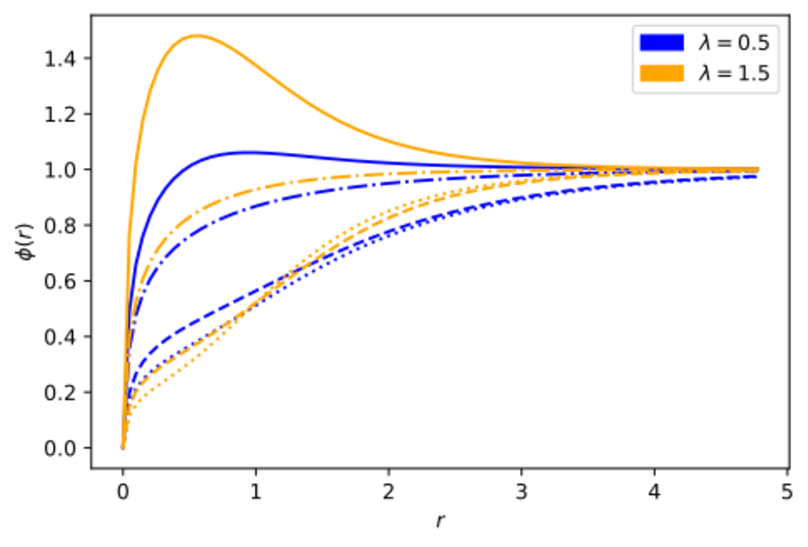
\includegraphics[width = 0.5\textwidth]{gfx/phi_gauss.pdf}}
	\subfloat[Campo de gauge $A_\theta(r)$.]{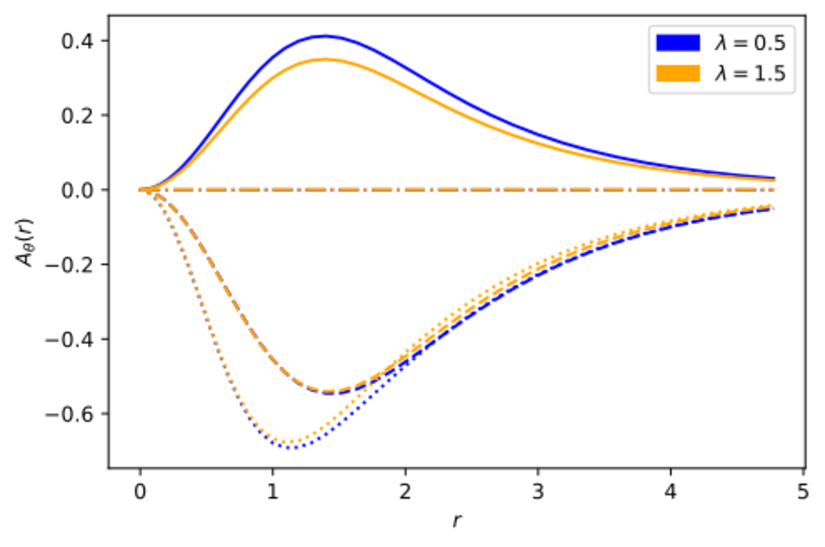
\includegraphics[width = 0.5\textwidth]{gfx/atheta_gauss.pdf}}
	\quad
	\subfloat[Energía de la configuración.]{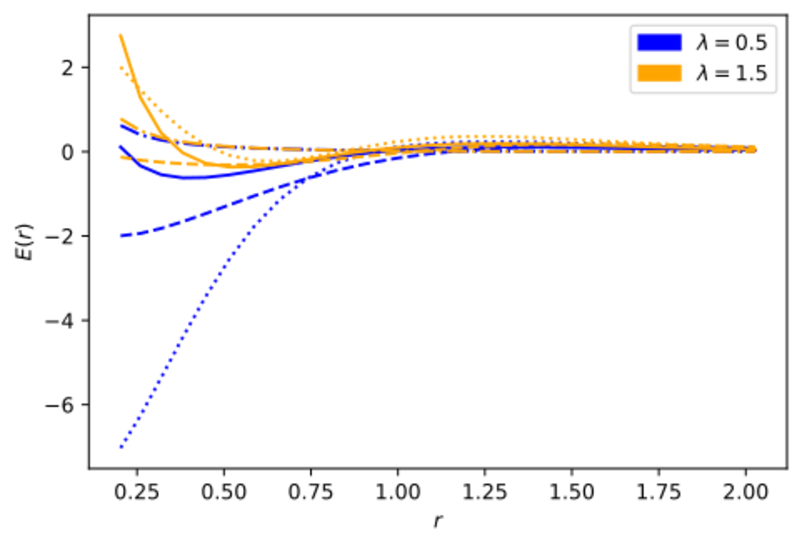
\includegraphics[width = 0.5\textwidth]{gfx/E_gauss.pdf}}
	\subfloat[Campo magnético.]{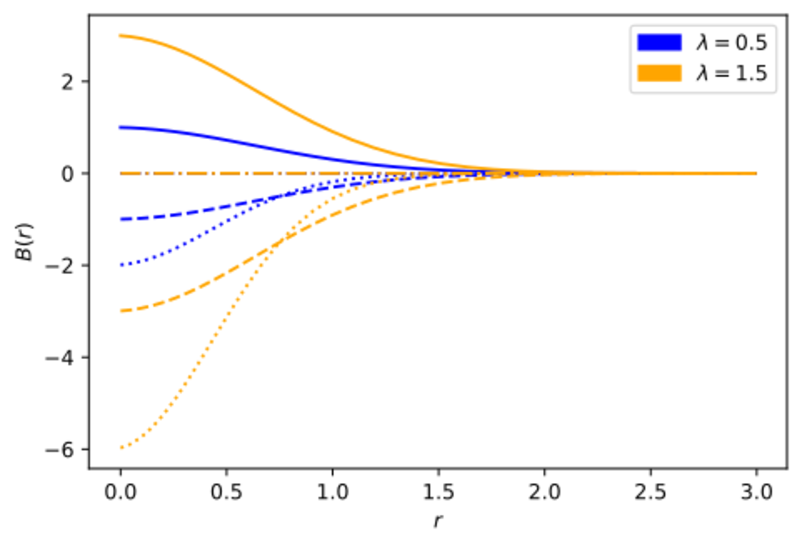
\includegraphics[width = 0.5\textwidth]{gfx/B_gauss.pdf}}
	\caption{Soluciones de vacío obtenidas minimizando numéricamente el potencial \eqref{eq:7.4.0.1}. Se muestra en azul las soluciones con $\lambda = 0.5$ y en naranja con $\lambda = 1.5$. Además, se muestran soluciones para distintas impurezas, a saber: $\sigma(r)=4 e^{-r^2}$ en líneas sólidas, $\sigma(r) = -4e^{-r^2}$ en líneas discontinuas y $\sg(r)=-8e^{-2r^2}$ en líneas punteadas. Como adicional, también se muestra las solución de vacío sin impurezas en líneas punteadas y discontinuas.}
	\label{fig:field_gauss}
\end{figure}

\begin{figure}[t]
	\centering
	\subfloat[Perfil del campo $\phi(r)$.]{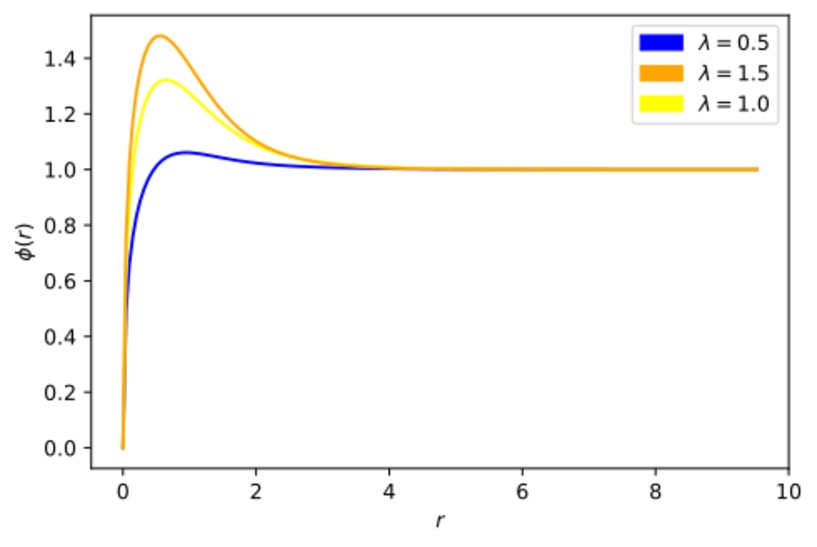
\includegraphics[width = 0.5\textwidth]{gfx/phi_lambdas.pdf}}
	\subfloat[Campo de gauge $A_\theta(r)$.]{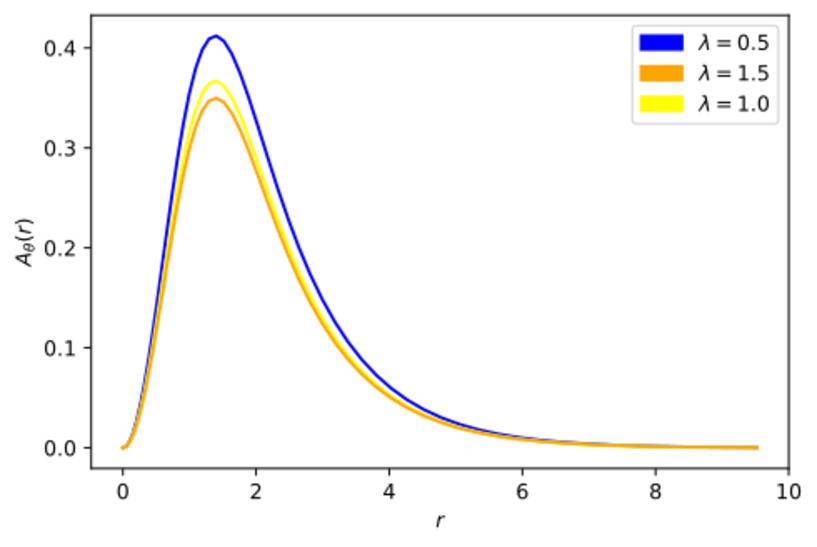
\includegraphics[width = 0.5\textwidth]{gfx/atheta_lambdas.pdf}}
	\quad
	\subfloat[Energía de la configuración.]{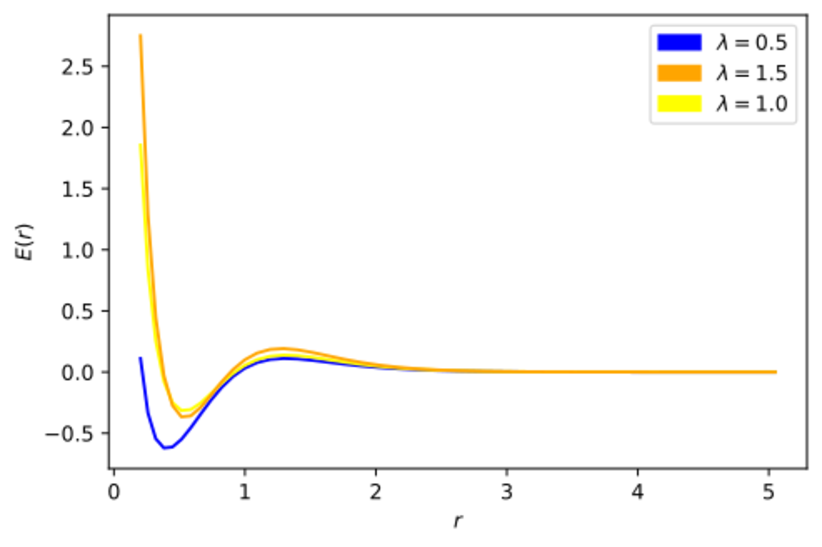
\includegraphics[width = 0.5\textwidth]{gfx/E_lambdas.pdf}}
	\subfloat[Campo magnético.]{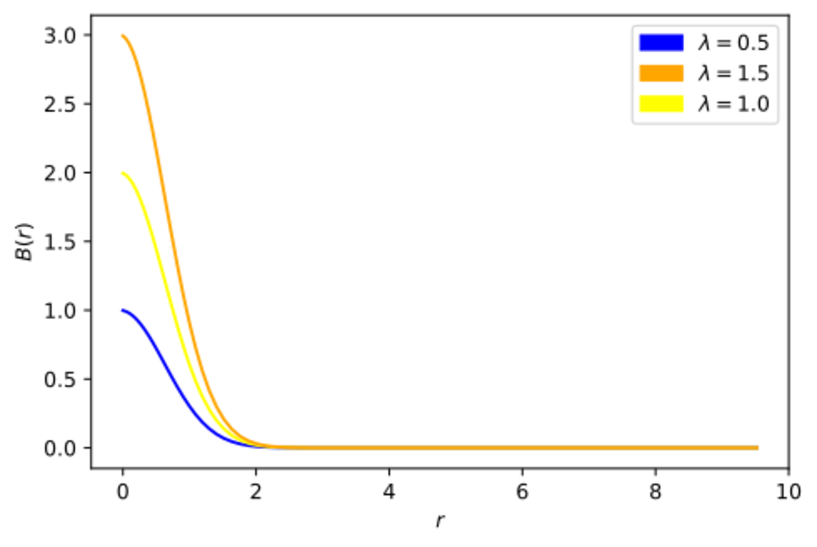
\includegraphics[width = 0.5\textwidth]{gfx/B_lambdas.pdf}}
	\caption{Soluciones de vacío obtenidas minimizando numéricamente el potencial \eqref{eq:7.4.0.1}. Se muestran soluciones para tres valores distintos de $\lambda$ en presencia de la impureza $\sg(r)=4e^{-r^2}$.}
	\label{fig:field_lambdas}
\end{figure}


